% -*- root: ../thesis.tex -*-
%!TEX root = ../thesis.tex
% ******************************* Thesis Chapter 2 ****************************


% ----------------------- paths to graphics ------------------------

% change according to folder and file names
\graphicspath{{2_background/figures/}}
% ----------------------- contents from here ------------------------

A short introduction to the basic theory of \acl{GPs} as well as their extension to large datasets using inducing points \cite{Titsias2009} is given in each paper on \ac{GPs}.
In this chapter, we go a bit more into the edetails of the basics of probabilistic Bayesian modeling, \acl{GPs}, \acl{VI} and sampling methods.


\section{Probabilistic Bayesian Modeling}

\label{sec:prob_bayes}

Bayes' theorem is one of the simplest theorem in probabilities and its demonstration fits in one line, yet its implications are \com{fill in word like "so important"}.

Let's give a very general modeling setting that we are going to follow for the rest of this chapter.
Given a set of observed variables $\bX$, a set of latent (unobserved) variables $\btheta$ with a \textit{prior} distribution $p(\btheta)$, and a \textit{likelihood} function $p(\bX\mid\btheta)$, we obtain the \textit{posterior} distribution $p(\btheta|\bX)$ via Bayes' theorem:
\begin{align}
p(\btheta|\bX) = \frac{p(\bX|\btheta)p(\btheta)}{p(\bX)} = \frac{p(\bX|\btheta)p(\btheta)}{\int p(\bX|\btheta)p(\btheta)d\btheta}
\label{eq:bayes}
\end{align}

The posterior allows us to obtain an estimate of the latent variables with its uncertainty given the prior $p(\btheta)$.
The posterior is used for computing all kind of expectations of the form $\expec{p(\btheta|\bx)}{f(\btheta)} = \int f(\btheta)p(\btheta|\bx)d\btheta$.
Expected values of interest can be statistics of the posterior like the mean $\expec{p(\btheta|\bx)}{\btheta}$ or predictions of new data points $p(\bx'|\bx) = \expec{p(\btheta|\bx)}{p(\bx'|\btheta)}$.

Probabilistic models can roughly be divided in two categories: \textbf{generative}, i.e. observed data has been generated from a stochastic model, and \textbf{discriminative}, i.e. observed data can be divided in two, typically input and output, and a stochastic model connects the two.
I will restrict the scope to discriminative models only.
Let's take the simple example of linear logistic regression, a discriminative model:
Given an input $\bx \in \mathbb{R}^D$ and binary label $y\in \{ 0, 1\}$, we model the generative model as:
\begin{align}
    y \sim \Be\left(\sigma(\btheta^\top \bx)\right),
\end{align}
where $\Be$ is the Bernoulli distribution, $\btheta\in\mathbb{R}^D$ and $\sigma$ is the logistic function $\sigma(x) = \frac{1}{1 + \exp(-x)}$, i.e. $\sigma : \mathbb{R} \mapsto [0, 1]$.
The likelihood function is given by: $p(y_i|\btheta,\bx_i) =\sigma\left(\btheta^\top \bx_i\right)^{y_i}\sigma\left(-\btheta^\top \bx_i\right)^{1-y_i}$ for an output label $y_i$ and input features $\bx_i$.
Given $\bX = \{\bx_1,\ldots,\bx_N\}$, $\boldy = \{y_1,\ldots,y_N\}$, the training data and the corresponding posterior $p(\btheta|\boldy, \bX)$ we can make predictions for new input data $\bx^*$:
\begin{align}
p(y^*|\bx^*,\boldy,\bX) = \int p(y^*, \btheta|\bx^*\boldy, \bX)d\btheta = \int p(y^*|\btheta,\bx^*) p(\btheta|\boldy,\bX)d\btheta.
\end{align}
Note that the last term of the equation directly involves the posterior distribution $p(\btheta|\by,\bX)$.
To solve this integral, we must either be able to both know the posterior in closed form and solve the integral numerically (or analytically), or be able to sample from it and compute this integral using Monte-Carlo integration.

\subsection{Posterior computations}
\label{sec:posterior}
Assuming that both the prior $p(\btheta)$ and the likelihood $p(\bx|\btheta)$ are known in closed-form, computing the posterior \eqref{eq:bayes} in closed-form involves computing the integral $p(\bx)=\int p(\bx|\btheta)p(\btheta)d\btheta$.
For most non-trivial models, this integral is intractable and approximations to the posterior and/or sampling approaches are needed.
These are introduced in Section~\ref{sec:approx_inf}.
However, in certain settings, computing the posterior in closed-form are possible.
This happens when the prior is said \textit{conjugate} to the likelihood, i.e. that the posterior is of the same probability distribution family as the prior.
If we consider the distributions part of the \textit{exponential family}, i.e. distributions that can be written as:
\begin{align}
    p(\btheta|\bphi) = h(\btheta)\exp(\boldeta(\bphi)^\top T(\btheta) - A(\bphi)),
    \label{eq:expfamily}
\end{align}
where $\bphi$ are the distribution parameters, $h(\btheta)$ is a \textit{base measure}, $\boldeta(\bphi)$ corresponds to the \textit{natural parameters}, $T(\btheta)$ are the sufficient statistics and $A(\bphi)$ is the \textit{log-partition}.
Note that any distribution can be written as an exponential family by using the trivial case where $p(\btheta) =h(\btheta)$.

Formally a \textit{conjugate prior} for a likelihood
\begin{align}
    p(\bx|\btheta) = h(\bx)\exp(\boldeta(\btheta)^\top T(\bx) - A(\btheta)),
    \label{eq:explikelihood}
\end{align}
is a distribution $p(\btheta|\balpha)$ defined as
\begin{align}
    p(\btheta|\balpha) = h'(\btheta)\exp(\boldeta'(\balpha)^\top T'(\btheta) - A'(\balpha)),
    \label{eq:expprior}
\end{align}
where $T'(\btheta) = \left\{\boldeta(\btheta), A(\btheta)\right\}$ and where $\balpha$ is the prior distribution parameters.
Given a factorizable likelihood $p(\bX|\btheta) = \prod_{i=1}^N p(\bx_i|\btheta)$, the posterior will be proportional to
\begin{align*}
    p(\btheta|\bX) \propto h'(\btheta)\exp\left(\left(\{\sum_{i=1}^N T(\bx_i), N\} + \boldeta'(\balpha)\right)^\top T'(\btheta)\right).
\end{align*}
The latter equation can easily be normalized since it is a known distribution.

Such conjugate models, are very practical and cheap to compute, but due to the constraints also tend to be too simple.
Without obtaining the posterior in closed-form it is sometimes possible to get all full-conditionals in closed-form, we can talk then about \textit{conditionally conjugate} models.
The full-conditional is defined as $p(\theta_i|\bx, \btheta_{/i})$ where $\btheta_{/i}$ represents the set of latent variables $\btheta$ where $\theta_i$ has been omitted.
Knowing the full-conditional distribution in closed-form means that when conditioned on the other variables, the posterior is known in closed-form.
What we need in practice is to be able to write the likelihood conditioned on the other  for each variable $\theta_i$ (or block of variables).
In the same exponential family example above, instead of looking for \eqref{eq:explikelihood}, we are interested in:
\begin{align*}
    p(\bx|\theta_i, \btheta_{/i}) = h(\bx, \btheta_{/i})\exp(\boldeta(\theta_i)^\top T(\bx, \btheta_{/i}) - A(\theta_i)).
\end{align*}

\section{Gaussian Processes}
\label{sec:gps}
\acf{GPs} are a class of stochastic processes used as non-parametric probabilistic representations to functions.
A \ac{GP} is a stochastic process $f_t$, where the joint distribution on any collection of variables $f_t$ follows a (multivariate) Gaussian distribution.
Their Gaussian nature makes them computationally very attractive.
Most operations on Gaussian variables can be done analytically, and they have other interesting properties (e.g. the marginal distribution of a component is also Gaussian). 
% The Gaussian distribution is to statistics what the harmonic oscillator is to physics".
\ac{GPs} are described to be a non-parametric, still one needs to define the covariance between each variable of the process.
\com{Missing transition}
One of the interpretation of a \ac{GP} is as a prior on functions in the \acf{RKHS}.
In practice the \ac{RKHS} is infinite-dimensional, and to be able to perform any computation one needs to project it into a finite-dimensional space.
Considering a function $f$ we wish to represent with a \ac{GP}, we can project it on data samples $\bX = \{\bx_i, \ldots, \bx_N\}$ and evaluate $f$ on them such that we obtain the finite-dimensional vector $\boldf$ where $f_i = f(X_i)$.
% \missingfigure{Put a prior of a GP}

One resorts to kernel functions % TODO need to cite this.
The kernel matrix $K$ is defined by $K_{ij} = k(x_i, x_j)$.
$K$ is positive-definite, i.e. for $K\in \real^{D\times D}$, and $x\in \real^D$, $x^\top K x > 0$.

\subsection{Gaussian Process Regression}

We now have a prior on the realization of the function $\boldf$ on the data $\bX = \{\bx_i\}_{i=1}^N$, $p(\boldf) = \No(\boldf|\bmu_0, \bK)$, where $\bmu_0 = \{\bmu_0(\bx_i)\}_{i=1}^N$ is the mean function.
We can add noisy observations $\by = \{y_i\}_{i=1}^N$ for each respective $\bX$:
\begin{align}
y_i = f(X_i) + \epsilon_i,
\end{align}
where $\epsilon_i \sim \No(0,\sigma^2)$.
This leads to the likelihood $p(y_i|f_i) = \No(y_i|f_i, \sigma^2)$.
Fortunately, multiplying Gaussian probability distributions together lead to another Gaussian distribution function.
The posterior for $\boldf$ is given by $p(\boldf|\by) = \No(\boldf|\by, \bK + \sigma^2 I)$.
The prediction of $f^*$ on a new point $\bx^*$ can be evaluated by computing:
\begin{align}
p(f^*|\bx^*,\bX,\by) = \int p(f^*|\boldf,\bx^*)p(\boldf|\bX,\by)d\boldf.
\end{align}	
This integral is analytically solvable and results in $p(f^*|\bx^*,\bX,\by)=\No(f^*|m^*,s^*)$ where $m^* = K_{\bx^*,\bX}(K_{\bX,\bX} + \sigma^{2}I)^{-1}\boldy$ and $s^*=K_{\bx^*,\bx^*} - K_{\bx^*,\bX}\left(K_{\bX,\bX}+\sigma^2I\right)^{-1}K_{\bX,\bx^*}$.

\begin{figure}
    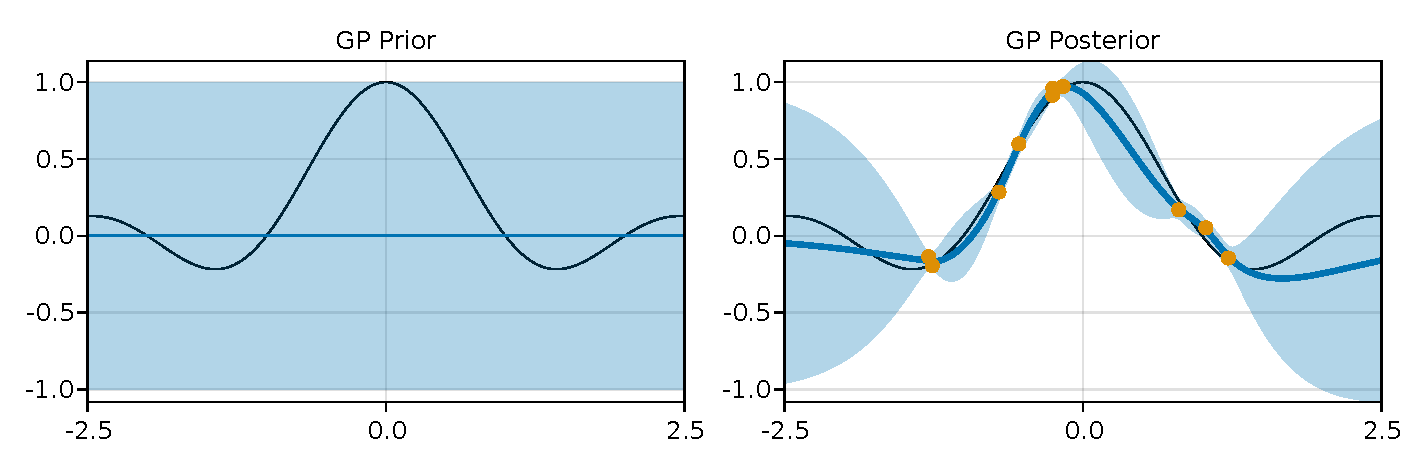
\includegraphics[width=\textwidth]{./chapters/2_background/figures/GP_example.pdf}
    \caption{Illustration of the realization of a Gaussian Process. The black is the true function, the blue line is the mean of the prediction, the blue area represent the confidence interval of 2 standard deviations, the orange points represent observed data. Left: prediction on a grid given no observations. Right: prediction on a grid given a set of observations}
    \label{fig:gp_example}
\end{figure}

\subsection{Non-Conjugate Gaussian Processes}

A Gaussian prior is only conjugate\footnote{A prior is said conjugate to a given likelihood when the resulting posterior is of the same family of the prior.} to a Gaussian likelihood
Therefore, \ac{GPs} only give a Gaussian posterior with a Gaussian likelihood, for all other cases we talk about \textit{Non-Conjugate Gaussian Processes}.
Examples of Non-Conjugate \ac{GPs} are binary classification, regression using non-Gaussian noise such as Student-t or Laplace noise.
Additionally, some likelihoods such as multi-class classification or heteroscedastic regression require multiple latent \ac{GPs}.

In all these cases, the posterior is not analytically tractable and one has to resort to the approximation methods presented in Section~\ref{sec:approx_inf}.

\subsection{Sparse Gaussian Processes}
One of the other largest issue of \ac{GPs}, regardless of the conjugacy of the likelihood, is the scalability with the number of observed samples.
When computing the covariance, the inverse operation has a computational complexity of $\mathcal{O}(N^3)$ where $N$ is the number of samples.
For one-dimensional inputs ($D=1$), solutions exist using state-space models representation, leading to an $\mathcal{O}(N)$ complexity but higher-dimensional problems require alternative solutions.
\citet{csato2002sparse} proposed first to create an approximation of the posterior using a subset of the points only in the context of online learning.
\citet{snelsonSparseGaussianProcesses2009} expanded this theory to the offline framework and \citet{Titsias2009} developed an alternative approximation based on KL divergence where the "inducing points" are not necessarily a subset of the training data and do not even have to belong to the same domain. \com{Cite related work}.

The rest of this thesis is based on \citet{Titsias2009} approach, where the approximation is made by defining a set of inducing points location $Z=\{\boldz_i\}_{i=1}^M$ and the respective realization of $\boldu$ where $u_i = u(\boldz_i)$
\begin{align}
    q(\boldu,\boldf) = q(\boldu)\prod_{i=1}^N p(f_i|\boldu)
    \label{eq:titsias_assumption}
\end{align}


\section{Approximate Bayesian Inference}
\label{sec:approx_inf}
The posterior distribution in Equation~\eqref{eq:bayes} cannot be computed in closed-form for non-trivial problems such as the one presented in Section~\ref{sec:gps}.
One can nonetheless to approximate the posterior to obtain a useful estimator for predictions and computing function expectations of interest.
This problem of \textit{Approximate Bayesian Inference} is a research field of its own, and this chapter will focus specifically on sampling and variational inference, the most used methods for \ac{GPs}.

\subsection{Sampling}

Even if the posterior distribution $p(\btheta|\bx)$ is not available in closed-form, one might be able to draw samples from it.
The whole collection of sampling techniques is again a whole research and the number of methods is too large to make mention of them all in this thesis.
Therefore, the scope will be restricted to methods favored or tailored to \ac{GPs}.
We will especially focus on \ac{MCMC} methods, where a
\subsubsection{Markov Chain Monte Carlo and Metropolis-Hastings}

\acf{MCMC} methods generate a chain of variables $\btheta^t$ with the Markov assumption: $\btheta^t$ depends only on $\btheta^{t-1}$ and where the stationary distribution of $\btheta^t$ is the same as the target distribution (for our use case the posterior $p(\btheta|\bx)$).
\ac{MCMC} methods require a transition probability $t(\btheta^{t+1}|\btheta)$ which leaves the target stationary distribution invariant, i.e. $p(\btheta) = \int t(\btheta|\btheta')p(\btheta')d\btheta'$.
Other properties such as detailed balance (a chain has the same probability to go backward and forward in time) and ergodicity (the chain should be able to explore all the parameter space and be aperiodic) need to be satisfied as well.

One the most common algorithm to run a Markov Chain sampling directly from a distribution $p(\btheta)$ is the \acf{MH} algorithm.
The \ac{MH} algorithm consists in having a proposal distribution $q(\btheta'|\btheta)$ suggesting a new sample.
Each proposed sample $\btheta'$ is randomly accepted or rejected with probability $p(\text{accept}) = A = \frac{p(\btheta')}{p(\btheta)}\frac{q(\btheta|\btheta')}{q(\btheta'|\btheta)}$.
The choice of the proposal distribution $q$ is the key to producing "good" chains with high acceptance rate and a good exploration of the parameter space of $\btheta$.
Next are presented briefly some important categories of choice for the proposal $q$.


\subsubsection{Gibbs Sampling}

Gibbs sampling is a particular \ac{MCMC} method where each random variable or block of random variables are sampled one after another separately.
The proposal distribution for the \ac{MH} algorithm is given by the full-conditional  $p(\theta_i|\bx,\btheta_{/i})$, where $\btheta_{/i}=\{\theta_1, \ldots \theta_{i-1}, \theta_{i+1},\ldots \theta_{D}\}$.
The biggest advantage of Gibbs sampling is that the acceptance probability is guaranteed to be 1:
\begin{align*}
    A =& \frac{p(\theta^{t+1}_i,\btheta^t_{/i}|\bx)}{p(\theta^t_i,\btheta^t_{/i}|\bx)}\frac{p(\theta^t_i|\bx,\btheta^{t}_{/i})}{p(\theta^{t+1}_i|\bx,\btheta^t_{/i})}\\
    =& \frac{p(\theta^{t+1}|\bx, \btheta^{t}_{/i})}{p(\theta^t_i|\bx,\btheta^t_{/i})}\frac{p(\btheta^t_{/i}|\bx)}{p(\btheta^t_{/i}|\bx)}\frac{p(\theta^t_i|\bx,\btheta^{t}_{/i})}{p(\theta^{t+1}_i|\bx,\btheta^t_{/i})} = 1.
\end{align*}
This means that all proposed samples are guaranteed to be accepted.
This process is illustrated on a two-dimensional bimodal example on Figure~\ref{fig:gibbs_samp}

\begin{figure}
\centering
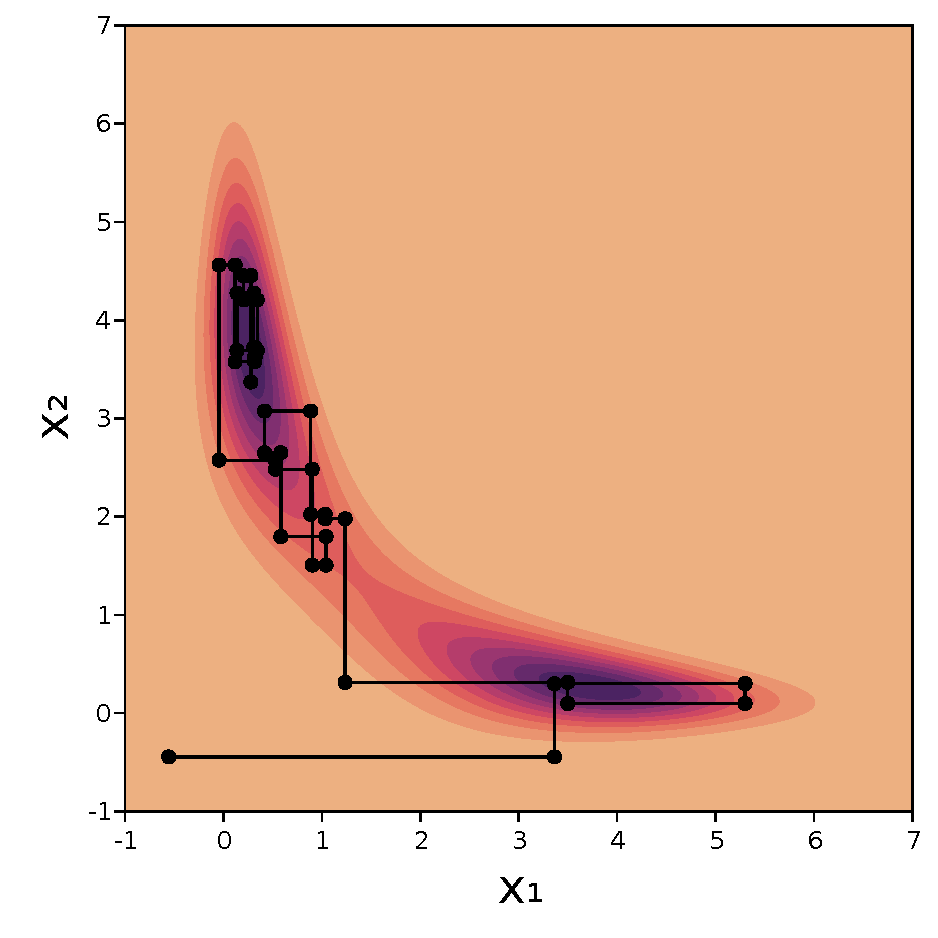
\includegraphics[width=0.5\textwidth]{./chapters/2_background/figures/gibbs_sampling.pdf}
\caption{20 steps of the Gibbs sampler trajectory on the Rosenbrock distribution in 2 dimensions}
\label{fig:gibbs_samp}
\end{figure}

However, the Gibbs sampling approach has several issues:
First, the full-conditional distribution is rarely available in closed-form and being able to sample from it is not always easy.
Second, there can be convergence issues if the variables are heavily correlated.
Some of these issues can be resolved by using additional techniques like "Blocked" Gibbs sampling \needcite where blocks of variables are sampled jointly or "Collapsed" Gibbs sampling \needcite where some variables are marginalized out from the full-conditional distribution.

\subsubsection{Hamilton/Hybrid Monte Carlo}

\acf{HMC} or Hybrid Monte Carlo \cite{betancourt2017conceptual} is a \ac{MCMC} gradient-based method.
Using Hamiltonian dynamics and augmenting the variables with a new momentum variables, one can guarantee both a high acceptance rate and a good exploration of the space.
\ac{HMC}'s proposal is to integrate the Hamiltonian dynamics with a randomly sampled momentum for a fixed number of steps with a given symplectic integrator.
Thanks to the energy conservation law, the acceptance rate is guaranteed to be close to 1, lower acceptance rates are due to numerical inaccuracies of the integrator.
\ac{HMC} has also multiple disadvantages: 
First, one needs to integrate differential equations based on gradients, which can be exceedingly expansive for some models.
Second, it has parameters to tune, namely the step size of the integrator, the number of steps taken and the metric matrix used.
Lastly, it only works for continuous variables.
For the second step automatic approaches exist, but they have their issues of their own as well.


\subsubsection{Elliptical Slice Sampling}

% TODO Finish this part


\subsection{Variational Inference}

\acf{VI}, also called Variational Bayes, consists in approximating the posterior $p(\btheta|\bx)$ with another distribution $q(\btheta)$.
Given a family of distributions $\mathcal{Q}$, parametrized by parameters $\bphi$ one aims to solve the following optimization problem:
\begin{align}
\bphi^* = \arg_{\bphi}\min \mathcal{D}\left(q_{\bphi}(\btheta), p(\btheta|\bx)\right),
\label{eq:prob_VI}
\end{align}
where $\mathcal{D}$ is a distance between two distributions and $q_{\bphi}$ is the distribution $q\in \mathcal{Q}$ parametrized by $\bphi$.
One of the most used distances is the backward \ac{KL} divergence, defined for continuous distributions as:
\begin{align}
\KL{q(x)}{p(x)} = \int q(x) \log \frac{q(x)}{p(x)}dx
\label{eq:kl}
\end{align}

The objective of Equation~\eqref{eq:prob_VI} or \eqref{eq:kl} is generally not directly tractable.
Since $p(\btheta|\bx)$ involves the normalization constant $p(\bx)$, one resorts to a surrogate function, the \ac{VFE} (or its negative counterpart the \ac{ELBO}):
\begin{align}
\KL{q_{\bphi}(\btheta)}{p(\btheta|\bx)} =& \int q_{\bphi}(\btheta) \left(\log q_{\bphi}(\btheta) - \log p(\btheta|\bx)\right)d\btheta\\
=&\int q_{\bphi}(\btheta) \left(\log q_{\bphi}(\btheta) - \log p(\btheta, \bx) - \log p(\bx)\right)d\btheta\\
=&\underbrace{- \log p(\bx)}_{\leq 0} + \int q_{\bphi}(\btheta) \left(\log q_{\bphi}(\btheta) - \log p(\bx|\btheta)- \log p(\btheta) \right)d\btheta\\
\leq& -\expec{q_{\bphi}}{\log p(\bx|\theta)} + \KL{q_{\bphi}(\btheta)}{p(\btheta)} = \VFE(\bphi)
\end{align}


By minimizing the \ac{VFE}, $\VFE(\bphi)$, instead of the \ac{KL} divergence, we can expect to find a solution close to the optimum of the problem stated in \eqref{eq:prob_VI}.

A standard way to find the $\bphi^* = \arg\min \VFE(\bphi)$ is to perform gradient descent on the variational parameters $\bphi$:
\begin{align}
\bphi^{t+1} = \bphi^{t} - \epsilon \grad_{\bphi}\VFE(\bphi^{t}).
\label{eq:vigraddescent}
\end{align}

Computing the gradient $\grad_{\bphi}\VFE(\bphi)$ can be non-trivial, as it involves derivatives over expectations.
Also, the choice of the family $\mathcal{Q}$ is a trade-off decision.
A richer, more complex family will probably be able to approximate the posterior better but computing the distance and optimizing will be increasingly difficult.
A standard example is the \ac{VGA}\footnote{The \ac{VGA} is explored in more details in Chapter~\ref{ch:chapter6}.}, i.e. the variational distribution $q_{\bphi}$ is a Gaussian, i.e. $\mathcal{Q} = \left\{q \sim \mathcal{N}(\boldm, S)\right\}$, and $\bphi = \{\boldm, S\}$.
One can decide to restrict $\mathcal{Q}$ further by specifying the structure of $S$.
Forcing it to be diagonal will simplify a lot of computations and avoid inverse operations, but all correlation information in the posterior will be completely lost.
This is what the mean-field approximation is about.

\subsubsection{Mean-Field Approximation}

One problem when considering $q_{\bphi}(\btheta)$ is that if we consider that all parameters are correlated to each other, the number of variational parameters to train grow quadratically with the dimensionality of $\btheta$.
The simplest assumption to add is the \ac{MF} approximation.
The \ac{MF} assumption is that every component of $\btheta$ to be independent of each other.
This variational family can be specified as $ = \left\{q | q \right\}$
\begin{align}
    \mathcal{Q}_{MF}= \left\{q = \prod_{i=1}^D q_{\bphi_i}(\theta_i)\right\},
\end{align}
where $\bphi_i$ are the variational parameters for the variable $\theta_i$.

One can also build more general distributions by considering independence between blocks of variables instead.
Given $\mathcal{I}=\{1,2,\ldots,D\}$, the set of indices of $\theta$, we can build into $K$ independent subsets $\mathcal{I}_k \subseteq \mathcal{I}$ such that  $\mathcal{I} = \cup_{k=1}^K \mathcal{I}_{k}$ and $\mathcal{I}_i \cap \mathcal{I}_j=\emptyset,~\mathrm{iff}~i \neq j$.
The variational distribution based on this \ac{BMF} approximation is then defined as
\begin{align}
    q^{BMF}_{\bphi}(\btheta) = \prod_{k=1}^K q_{\bphi_k}(\btheta_{\mathcal{I}_k}),
\end{align}
where $\bphi_k$ are the variational parameters for the set of variable $\btheta_{\mathcal{I}_k}$.

\subsubsection{Coordinate Ascent VI}

Based on the \ac{MF} and \ac{BMF} approach, we are interested in finding the solution for each set of parameters $\bphi_i$ to
\begin{align}
    \bphi_i^* = \arg_{\bphi_i}\min \VFE(\bphi_i, \bphi_{/i}),
    \label{eq:optimalbphi}
\end{align}
i.e. by keeping all other parameters fixed, what is the optimal $\bphi_i^*$.
This can be found either by solving
\begin{align}
\left.\grad_{\varphi_i}\VFE(\bphi)\right\vert_{\varphi_i=\varphi_i^*} = 0,
\end{align}
or performing the same gradient scheme as \eqref{eq:vigraddescent}.
In some cases the solution to \eqref{eq:optimalbphi} is given by
\begin{align}
q_{\bphi_i}^*(\btheta_i) \propto \exp\left(\expec{q_{\bphi}(\btheta_{/i})}{\log p\left(\btheta_i|\btheta_{/i},\bx\right)}\right)
\end{align}
where $\btheta_{/i}$ represent the collection of variables $\btheta_{/i} = \{\theta_j | j \neq i\}$.
The distribution $p(\btheta_i|\btheta_{/i},\bx)$ is the full-conditional distribution as described in Section~\ref{sec:posterior}.

When working with distribution coming from exponential families, it is straightforward to get the optimal variational parameters $\bphi$.
By updating the parameters one after another we get a \ac{CAVI} scheme\footnote{The word ascent is used since the scheme was originally derived using the negative \ac{VFE} i.e. the \ac{ELBO}.}.
Effectively, one updates each variational parameter $\bphi_i$ with its optimum given the rest of the variational parameters $\bphi_{/i}$ via closed-form functions:
\begin{align}
\varphi_i^{t+1} = f_i\left(\bphi_{1:(i-1)}^{t+1}, \bphi_{(i+1):D}^t\right).
\end{align}
The order of the updates do not matter as long as the variational parameters $\bphi$ are initialized in their domain.

The full algorithm is presented on Algorithm~\ref{alg:CAVI}.

\begin{algorithm}
    \caption{\ac{CAVI} Updates}
    \label{alg:CAVI}
    \begin{algorithmic}
        \While {$|\VFE^{t+1} - \VFE^t| > \epsilon$}
            \ForAll {$i \in \{1,\ldots,D\}$}
                \State $\bphi_i^{t+1} = f_i\left(\bphi_{1:(i-1)}^{t+1}, \bphi_{(i+1):D}^t\right).$
            \EndFor
        \EndWhile
    \end{algorithmic}
\end{algorithm}


\subsubsection{Natural Gradients}

One interesting aspect of \ac{CAVI}, is that it implicitly uses \textit{natural gradients} \cite{amariNaturalGradientWorks1998}.
A natural gradient is a gradient preconditioned with the inverse Fisher information matrix defined as
\begin{align}
    \mathcal{I}_\theta = \expec{p(\bx|\btheta)}{\left(\grad_{\btheta}\log p(\bx|\btheta)\right)\left(\grad_{\btheta} \log p(\bx|\btheta)\right)^\top} = -\expec{p(\bx|\btheta)}{\mathbf{H}(\log p(\bx|\btheta))},
    \label{eq:fisherinfomatrix}
\end{align}
where $\mathbf{H}(f)$ is the Hessian matrix of the function $f$.
The Fisher information matrix is a Riemannian metric which gives the direction of the steepest descent with respect to the KL divergence.
\com{Give more details about the meaning of the Fisher info}
The natural gradient is given by :
\begin{align*}
    \widetilde{\grad}_{\bphi}\mathcal{F}(\bphi) = \mathcal{I}^{-1} \grad_{\bphi}\mathcal{F}(\bphi)
\end{align*}
The natural gradient is constructed such that the metric it gives maximizes the change of the \ac{KL} divergence between the given distribution and its target.
The reason why natural gradients are brought up here is that the updates of the \ac{CAVI} algorithm \ref{alg:CAVI} for exponential distributions, can be interpreted as natural gradient ascent updates with learning rate $1$.
\begin{align*}
    \bphi^{t+1} = \bphi^t + \mathcal{I}^{-1}\grad_{\bphi}\mathcal{F}(\bphi^t) \equiv \bphi^{t+1}
\end{align*}


\subsection{Scale-Mixtures and conditionally conjugate likelihoods}
\label{sec:scale-mixtures}
A large part of this work is based on scale-mixtures and mixtures in general.
A scale-mixture is a continuous mixture of a distribution with a varying scale parameter.
A textbook example is the Student-T distribution which is a Gaussian scale-mixture with a Gamma distribution on the scale weights:
\begin{align*}
    T_\nu(x) = \int_{0}^\infty \mathcal{N}\left(x|0,\omega\right)\mathrm{Ga}\left(\omega|\frac{\nu}{2}, \frac{\nu}{2}\right)d\omega,
\end{align*}
where $\mathrm{Ga}$ is a Gamma distribution.
Another example is the Laplace distribution which is also a Gaussian scale-mixture:
\begin{align*}
    \mathrm{La}(x|\beta) = \int_0^{\infty} \mathcal{N}(x|0,\omega)\mathrm{Exp}\left(\omega|\frac{1}{2b^2}\right)d\omega,
\end{align*}
where $\mathrm{Exp}$ is the exponential distribution.

Generally these representations are used to compute predictive distributions.
For example in linear regression with a Gamma prior on the likelihood variance, the resulting posterior predictive distribution will be a Student-T distribution.
In this thesis we show that we can use this connection the other way around.
Given a likelihood $p(\bx|\btheta)$ which can be defined as a marginalized scale-mixture,
we can \textit{augment} the likelihood by "ummarginalizing" the scale-mixture.
We transform for example a Student-T likelihood into a Gaussian likelihood with a Gamma prior.
This allows for so-called conditionally conjugate likelihoods.


Now that all important and necessary topics for this thesis have been overviewed, the following will present the different works presented in this thesis. 
% ---------------------------------------------------------------------------
% ----------------------- end of thesis sub-document ------------------------
% ---------------------------------------------------------------------------